
\subsection{The Ride to the Airport}

The Uber was a black Escalade with cooled leather seats and the faint smell of eucalyptus from a vent 
clip in the dash. David climbed in, offered a nod to the driver, and settled into the backseat. The 
city outside was still shaking off the morning: joggers with earbuds, cafes flipping signs, and garbage 
trucks doing their work like it mattered.

David opened his laptop.

Slide 14 greeted him again, unchanged from the night before:
\textit{Risk Stratification Under Uncertainty.}

But now he had to move faster.

He wasn’t behind because of laziness. He was behind because of pancakes. Because of syrup. 
Because his son had asked if he could stay just five more minutes... and he had.

So here he was, revising in transit, because he chose to make breakfast.

And even with the mounting pressure, he didn’t regret it.

He clicked through his deck with the methodical pace of a surgeon reviewing x-rays. Slide by slide, the story emerged
about how his startup could automate the soul-crushing grind of regulatory compliance.

Not just dashboards or alerts.

\textit{Narrative automation. Report generation. Fully auditable traceability.}

Because financial institutions were required to submit mountains of documentation to regulators, and while the 
rules varied slightly across jurisdictions — Basel, Dodd-Frank, ESMA, MAS — the structural bones were always the same:
\textbf{classify, justify, certify}.

\medskip

\begin{HistoricalSidebar}{A Brief History of Financial Regulation Reporting}

    Modern financial reporting requirements are the aftershocks of crisis.
    
    \medskip
    
    After the 1929 stock market crash, the U.S. passed the \textbf{Securities Act of 1933} and the 
    \textbf{Securities Exchange Act of 1934}, giving rise to the SEC and enshrining the principle 
    of disclosure: \textit{you don’t have to be honest, but you do have to report what you’re doing 
    so someone can check}. Annual 10-Ks, quarterly 10-Qs, and a cascade of schedules followed.
    
    \medskip
    
    In the decades that followed, regulation often lagged innovation. Derivatives exploded in the '80s. 
    Risk reporting didn’t catch up until the \textbf{Basel Accords}, a series of international banking 
    standards set by the Basel Committee beginning in 1988. Basel I introduced capital requirements. 
    Basel II added “risk-weighted assets.” Basel III came after the 2008 financial crisis and emphasized 
    stress testing, liquidity coverage, and leverage ratios. Each step added layers of required documentation 
    — and interpretive gray zones.
    
    \medskip
    
    Meanwhile, the U.S. Dodd-Frank Act of 2010, passed in the wake of the global financial crisis, created 
    more than 400 new rules and mandated detailed documentation of systemic risk, trading activity, third-party 
    exposure, and internal controls. Institutions had to file Form PFs, living wills, swap data reports, and 
    CCAR submissions. Europe responded with its own: \textbf{MiFID II}, \textbf{EMIR}, \textbf{CRD IV}.
    
    \medskip
    
    But no matter the jurisdiction, the workflow was the same:

    \medskip

    \begin{enumerate}
    \item \textbf{Classify} the assets and exposures.
    \item \textbf{Justify} the risk methodologies and controls.
    \item \textbf{Certify} compliance through formal attestation and documentation.
    \end{enumerate}
    
    \medskip
    
    Regulators didn’t demand certainty — they demanded \textit{coherence}. And that meant narrative. Every 
    number had to be explained. Every position had to be defended.
    
    \medskip
    
    By the 2020s, the volume of regulatory reporting had grown so massive that it quietly spawned an entire 
    cottage industry — RegTech — with startups offering software to automate filings, format disclosures, and 
    validate transaction records.
    
    \medskip
    
    But David’s insight went a step further:
    \textbf{What if the reports didn’t just comply with regulation? What if they interpreted it too?}

    \medskip
    
    Because the regulators weren’t just asking for answers.
    They were asking if you understood the question.

\end{HistoricalSidebar}

\medskip

The vast majority of compliance reporting was standarized. It was repetition.
Same tables. Same language. Same formatting.
Most risk officers were glorified stenographers who copy structured data from one box into another.
However, that's not the hard part. The hard part is making sense of the data.

The regulation, David liked to say, was scripture.
And scripture is interpreted.

So David's solution was simple:
\textbf{train a model to interpret the scriptures faster than the priests.}

His slides detailed the pipeline.

\medskip

\begin{figure}[H]
    \centering
    \resizebox{0.85\textwidth}{!}{%
      \begin{tikzpicture}[
        font=\footnotesize,
        stage/.style={draw=black, thick, rounded corners, minimum width=3.6cm, minimum height=1.6cm, align=center, fill=gray!10},
        arrow/.style={->, thick},
        node distance=1.5cm and 2.6cm
      ]
  
      % Top Row (left to right)
      \node[stage] (extract) at (0,0) {
        \parbox{3.4cm}{
            \centering \textbf{Extract} \\\ \\
            \begin{itemize}
                \item Transaction logs 
                \item Margin calls
            \end{itemize}
          }
      };
  
      \node[stage, right=of extract] (model) {
        \parbox{3.4cm}{
            \centering \textbf{Interpret} \\\ \\
            \begin{itemize}
                \item Risk heuristics
                \item Data context
            \end{itemize}
        }
      };
  
      % Downward arrow to next tier
      \node[stage, below=2.2cm of model] (generate) {
        \parbox{3.4cm}{
            \centering \textbf{Generate Narrative} \\\ \\
            \begin{itemize}
                \item Summaries 
                \item Analysis
            \end{itemize}
        }
      };
  
      \node[stage, left=of generate] (deliver) {
        \parbox{3.4cm}{
            \centering \textbf{Deliver} \\\ \\ 
            \begin{itemize}
                \item PDFs 
                \item Audit trails
            \end{itemize}
        }
      };
  
      % Arrows
      \draw[arrow] (extract) -- (model);
      \draw[arrow] (model) -- ++(0,-1.2) -- (generate.north);
      \draw[arrow] (generate) -- (deliver);
  
      \end{tikzpicture}%
    }
    \caption{Slide Snapshot: Snake-style pipeline from data extraction to regulatory narrative delivery.}
\end{figure}

\medskip

Most RegTech startups solved for formatting.

They offered tools that ingested data, standardized it across jurisdictions, and outputted XML or JSON 
in regulator-approved schemas. They built dashboards that tracked deadlines, flagged anomalies, and 
generated templated disclosures based on pre-defined rules.

But their systems were reactive.

They followed the letter of compliance, and not its spirit. They automated checklists, not judgment. Their 
``AI'' was often just glorified decision trees hidden behind polished UIs.

\medskip

\begin{figure}[H]
    \centering
    \resizebox{0.85\textwidth}{!}{%
      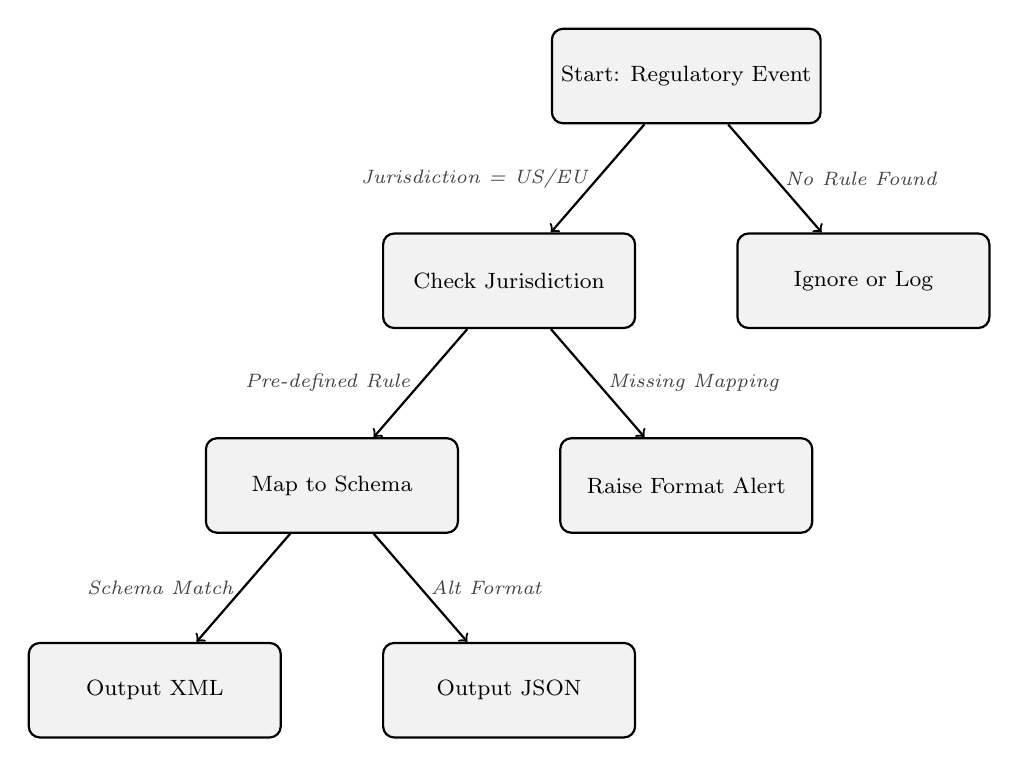
\begin{tikzpicture}[
        font=\footnotesize,
        node/.style={draw, rounded corners, align=center, minimum width=3.2cm, minimum height=1.2cm, fill=gray!10, thick},
        edge from parent/.style={draw, thick, ->},
        level distance=2.6cm,
        sibling distance=4.5cm,
        metadata/.style={font=\scriptsize\itshape, text=gray!50!black}
      ]
  
      \node[node] {Start: Regulatory Event}
        child { node[node] {Check Jurisdiction}
          child { node[node] {Map to Schema}
            child { node[node] {Output XML} 
              edge from parent node[midway, left, metadata] {Schema Match} }
            child { node[node] {Output JSON}
              edge from parent node[midway, right, metadata] {Alt Format} }
            edge from parent node[midway, left, metadata] {Pre-defined Rule}
          }
          child { node[node] {Raise Format Alert}
            edge from parent node[midway, right, metadata] {Missing Mapping}
          }
          edge from parent node[midway, left, metadata] {Jurisdiction = US/EU}
        }
        child { node[node] {Ignore or Log}
          edge from parent node[midway, right, metadata] {No Rule Found}
        };
  
      \end{tikzpicture}%
    }
    \caption{Illustrative Decision Tree: A simplified RegTech compliance system built on pre-defined rules and 
    deterministic formatting logic.}
\end{figure}

\medskip

David’s pipeline was different.

It wasn’t just built to file forms. It was built to reason.
Where startups parsed static fields, David’s models digested narrative.
Where others validated with if-statements, he mimicked analyst intuition.
Where others summarized in bullets, he wrote paragraphs in the voice of a junior compliance officer.
And most critically, where others stopped at formatting, he captured \textit{justification}.

Because he understood what most vendors didn’t.
\textbf{Regulators don’t want answers. They want accountability in prose.}

\medskip

\begin{HistoricalSidebar}{Scripture, Commentary, and the Politics of Interpretation}

    Religious texts are not read. They are interpreted.
    And interpretation, throughout history, has been the real seat of power.
    
    \medskip
    
    The \textbf{Qur’an}, for instance, is considered by Muslims to be the literal word of God. But its 
    application in everyday life is shaped not just by the Qur’an itself, but by the \textbf{Hadiths} --- 
    collections of sayings and actions of the Prophet Muhammad --- and by generations of \textbf{tafsir} 
    (interpretive commentary) authored by scholars, jurists, and theologians.
    
    \medskip
    
    Similarly, the \textbf{Torah} — the foundational text of Judaism — is accompanied by layers of 
    interpretive tradition, including the \textbf{Mishnah}, \textbf{Talmud}, and countless rabbinical commentaries. 
    Jewish legal rulings (halakha) don’t come directly from the Torah, but from how generations of rabbis 
    debated and interpreted its words.
    
    \medskip
    
    Even the Protestant Reformation wasn’t a dispute over which Bible to read. It was a dispute over how to 
    interpret it. \textbf{Luther} and \textbf{Calvin} read the same scriptures. But their commentaries ---
    their theological models --- diverged in ways that reshaped Europe.  

    \medskip
    
    The difference wasn’t in the text. It was in the narrative applied to it.
    
    \medskip
    
    David understood this intuitively.

    \medskip
    
    \textit{Regulation is scripture.} And scripture must stay within the accepted bounds of interpretation.
    
    \medskip
    
    His LLM wasn’t generating answers. It was generating \textbf{commentary}.
    Narratives that mirrored the voice of the compliance priesthood, but faster, cheaper, and more reliably.

    \medskip
    
    Like Luther with a printing press, David was automating the reformation.
    
\end{HistoricalSidebar}

\medskip

Unlike most RegTech platforms --- which focus on formatting data into regulator-approved schemas and automating 
checklist-driven tasks --- David’s system aimed to replicate judgment, not just structure. 

Traditional tools ingested 
data, standardized it, and outputted XML or JSON files with rule-based templates, often powered by decision trees 
disguised as intelligence. In contrast, David’s pipeline began by extracting structured data from transaction logs, 
margin calls, and trading desk summaries. However, what followed was fundamentally different. Instead of routing that 
data through static logic, it passed through a machine learning model designed to mimic the interpretive heuristics 
of a junior compliance analyst, identifying not just what was present, but what mattered. 

The system then generated full narrative summaries --- not bullet points --- using fine-tuned large language models 
trained to speak in regulatory 
tone, operating within memory constraints and guided by feedback loops. 

The final product wasn’t just compliant; it 
was coherent: regulator-ready PDFs embedded with audit trails that didn’t just prove the math ---  they explained 
the reasoning.

\medskip

\begin{PhilosophicalSidebar}{Hermeneutics --- From Scripture to Systems}

    Hermeneutics — the theory and methodology of interpretation — has its roots in theology.
    
    \medskip
    
    After the Protestant Reformation fractured the authority of the Catholic Church, a pressing question emerged:  
    \textbf{If we all have the same Bible, why do we read it so differently?}
    
    \medskip
    
    With centralized dogma destabilized, scholars and theologians needed new tools to adjudicate meaning. Thus, 
    hermeneutics matured into a discipline: not just \textit{what} the text said, but \textit{how} it was read.  
    Different sects developed distinct interpretive lenses — historical, allegorical, moral, and anagogical — 
    in an effort to ground their doctrines in reason rather than tradition.


    \medskip

    For example, in 1615, Galileo wrote a letter to the Grand Duchess Christina of Tuscany to explain why 
    heliocentrism didn’t contradict the Bible. His argument? Scripture wasn’t meant to teach physics; it was 
    meant to teach salvation. So if the Bible said “the sun stood still,” it was speaking in the language of 
    everyday experience, and not making a scientific claim. 

    \medskip
  
    Galileo argued that God gave us two books: \emph{the Bible and the Book of Nature}. And since God doesn’t 
    contradict Himself, any contradiction between science and scripture meant we were interpreting one of 
    them wrong. (Spoiler: he thought it was the theologians who needed to rethink things.)
  
    \medskip
  
    \textbf{This was not a crazy position.} Saint Augustine and Thomas Aquinas had both warned against 
    reading the Bible too literally in matters of natural philosophy. But Galileo was making this argument 
    during the height of the Counter-Reformation, when the Catholic Church was cracking down on anything 
    that sounded even remotely Protestant (including interpreting the Bible for yourself). 
    
    \medskip
    
    But hermeneutics didn’t stay in the church.
    
    \medskip
    
    In the 20th century, philosopher Martin Heidegger redefined hermeneutics — the art of interpretation — as a 
    fundamental structure of human existence. In Being and Time, he introduced the concept of Dasein: the being for 
    whom being is a question, and whose very mode of existence is interpretive. For Heidegger, interpretation wasn’t 
    a scholarly exercise reserved for theologians or literary critics. It was existential. 

    \medskip
    
    We don’t encounter raw facts, he argued; we encounter meaning, always already filtered through our situation, 
    language, and historical context. 

    \medskip
    
    What’s less commonly discussed is that Heidegger began his intellectual life as 
    a Catholic seminarian. He studied theology and read Martin Luther closely, and absorbed the Protestant reformer’s 
    radical approach to the Bible. Though Heidegger eventually lost his religious faith, he retained Luther’s hermeneutic 
    stance and universalized it: applying it not just to scripture, but to law, literature, ritual, and even technology. 
    In his hands, hermeneutics escaped its theological origins and became a method for understanding all systems of 
    meaning whether legal codes, social norms, computer user interfaces, and machine logic.
    
    \medskip
    
    \textbf{David’s insight?}  
    That regulatory compliance --- like scripture --- isn’t just about rules.  
    It’s about how those rules are read, applied, and justified.
    
    \medskip
    
    So when he trained his models to \textit{interpret the scriptures faster than the priests},  
    he wasn’t automating compliance.  
    He was building an interpretive machine.
    
\end{PhilosophicalSidebar}

\medskip


One slide showed a side-by-side:
\textit{Human-Generated Report (3 hrs)} vs. \textit{LLM-Generated Report (13 seconds)}.
The differences were indistinguishable. He’d tested it on ex-regulators. They didn’t spot the swap.

Another slide bore the heading:

\begin{quote}
    \centering
    \textbf{The Paradox of Compliance: Everyone’s Accountable, And No One Wants to Write It.}
\end{quote}

He smiled at that one.

The deck ended with a quote he planned to use onstage:
\textit{“The cost of compliance is not risk. It’s attention.”}

David leaned back, exhaled, and let the screen dim.

He loved his family.
It wasn’t an empty claim. It wasn’t PR. It was bone-deep.
Every decision he made — every corner he cut, and every night he worked past exhaustion — was for them.

And it hurt. God, it hurt.
To miss the little moments. To feel the space widening between himself and Emma.
To wonder whether his kids would remember him more for his presence or his promises.

But he told himself --- as he had every day for the past three years --- that it would be worth it.
That one day, when it all worked, they’d look back and understand.

He had chosen to make breakfast.
And now he was choosing to work.

That, to him, was love.

The SUV merged onto the expressway.
David reopened his laptop.
Slide 17 still needed polish.

\subsection*{Editor Questions for ``The Ride to the Airport''}

This scene blends personal reflection with technical ambition, using the quiet of a car ride to reveal both professional vision and emotional sacrifice. These questions aim to help probe that intersection: where love, work, and narrative automation collide. Focus on what landed — and what didn’t quite reach.

\subsubsection*{Narrative \& Structure}

\begin{itemize}
  \item Did the pacing feel natural given the blend of technical exposition and emotional reflection?
  \item Did the “ride to the airport” serve as an effective setting for this internal and thematic arc?
  \item Were the historical and philosophical sidebars integrated smoothly, or did they interrupt the emotional flow?
\end{itemize}

\subsubsection*{Emotional Resonance}

\begin{itemize}
  \item Did David’s internal conflict (family vs. mission) feel authentic and earned?
  \item How did the pancake reference echo emotionally throughout the scene? Did it deepen your empathy?
  \item Did his justification for working — that “choosing to work is love” — feel resonant, tragic, rationalized, or something else?
\end{itemize}

\subsubsection*{Character Insight}

\begin{itemize}
  \item What did this scene reveal about David’s relationship with his family that prior scenes hadn’t?
  \item Did David feel more sympathetic, more driven, or more disconnected after this scene?
  \item Was there a line or moment that sharpened your understanding of his psychological makeup?
\end{itemize}

\subsubsection*{Thematic Depth}

\begin{itemize}
  \item How well did the metaphor of regulation as scripture land for you?
  \item Did the historical/philosophical parallels (hermeneutics, Reformation) feel pretentious, powerful, or illuminating?
  \item What deeper theme do you think this scene is exploring: automation, interpretation, fatherhood, control, guilt?
\end{itemize}

\subsubsection*{Scene Texture \& Craft}

\begin{itemize}
  \item Did the specific details (eucalyptus scent, slide titles, syrup memory) enhance the realism?
  \item Was there a line or transition that felt especially elegant or jarring?
  \item Did the final image (laptop reopening) feel like a satisfying close or a setup for what’s next?
\end{itemize}

\subsubsection*{Sidebars and Integration}

\begin{itemize}
  \item Did the historical and philosophical sidebars deepen your engagement with the scene — or distract from it?
  \item Would you prefer these insights to be embedded in David’s inner monologue rather than set apart?
  \item Was there a moment where the historical sidebar felt particularly aligned (or misaligned) with the narrative’s emotional arc?
\end{itemize}

\subsubsection*{Deeper Testing}

\begin{itemize}
  \item What would be lost if this scene were cut — emotionally or structurally?
  \item If this were the first time you met David, what impression would you walk away with?
  \item If you had to summarize this scene in one word, what would it be?
\end{itemize}